\chapter{Stand der Technik}
\section{Vorarbeiten zur Bachelorthesis}
Zum Thema dieser Bachelorarbeit wurden bereits zwei Vorarbeiten geleistet. Zum einen wurde im Rahmen einer Praxisphase, eine Voruntersuchung zum Thema \textit{Condition-Based-Monitorig für industrielle PCs}  vorgenommen. Die im Rahmen der Arbeit \cite{PAMathias} durchgeführte Grundlagenuntersuchung und Marktrecherche hat auf zwei Computer Monitoring Technologien aufmerksam gemacht. Diese wurden anschließend in der zweiten Vorarbeit \cite{t3000} evaluiert. Aus dieser Bewertung heraus, wurde sich für die \textit{HWiNFO} Software, zum Auslesen der auf der Hardware verbauten Sensorik entschieden. Die Software wird genauer in Abschnitt \ref{sec:HWiNFO} behandelt. Des Weiteren wurde in der Vorarbeit \cite{t3000} auch eine geeignete Datenbank für das Health Monitoring System ausgewählt. In Abschnitt \ref{sec:SQLite} wird die ausgewählte Datenbanktechnologie genauer beschrieben. 

\subsection{SQLite Embedded Datenbank}\label{sec:SQLite}
In der Vorarbeit \cite{t3000} zu dieser Bachelorarbeit wurde eine Auswahl für eine Datenbank getroffen. Hierzu wurden drei Datenbanken in den Punkten Performanz, Größe der Anwendung, Ressourcennutzung und der Dokumentation miteinander verglichen. Die Resultate werden in der Entscheidungs Matrix \ref{fig:MatrixDB} aufgeführt. Aus dem Vergleich  hervorgehend, wurde sich für die Verwendung der SQLite Embedded Datenbank Engine entschieden. Diese bietet eine zuverlässige, kleine, schnelle und voll funktionale Datenbank Engine, welche vollständige in das Gesamtsystem integriert werden kann \cite{SQLiteHompage}. Zur Implementierung der Datenbank in die Anwendung wird die System.Data.SQLite Bibliothek für C\# verwendet.\\ 
Auf das Thema Datenbanken wird in Abschnitt \ref{sec:Datenbank} genauer eingegangen.
\begin{flushleft}
    \begin{figure}[h!]
        \centering
        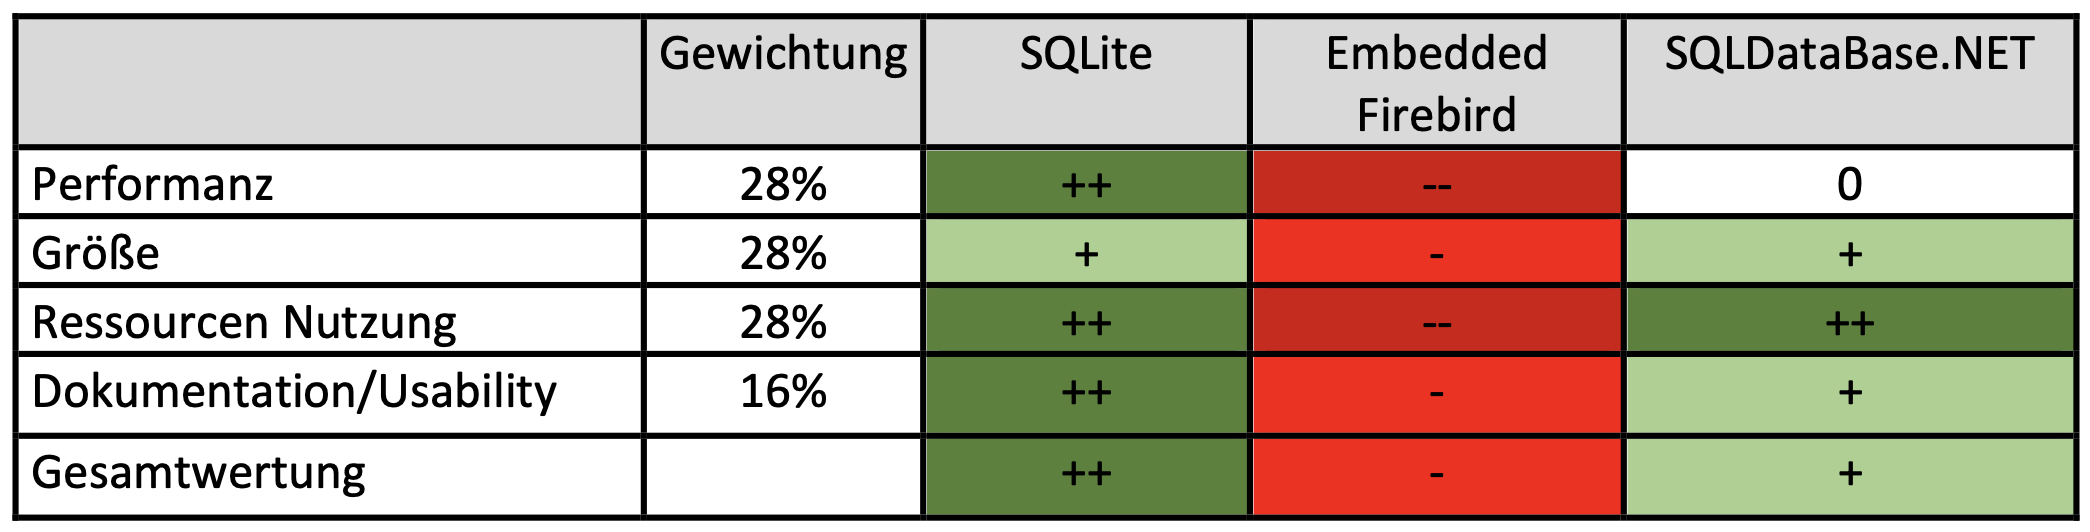
\includegraphics[width=1\linewidth]{MatrixDB}
        \caption{Entscheidungs Matrix zur Bewertung der Datenbanken \cite{t3000}}
        \label{fig:MatrixDB}
    \end{figure}
\end{flushleft}
\vspace{-2cm}
\subsection{HWiNFO}\label{sec:HWiNFO}
\textit{HWiNFO} ist eine Software der Firma REALiX, welche zum Überwachen und Analysieren der Hardware eines Computers konzipiert wurde \cite{HWINFO}. Über die grafische Oberfläche des Programms, lassen sich alle gesammelten Daten anzeigen. Der Nutzer kann diese Informationen nutzen, um Defekte an der Hardware zu erkennen.\\
Das ausschlaggebende Argument für die Nutzung der Software liegt in der \ac{api}. Über die Shared Memory Funktion der Software lassen sich alle Gerätedaten, die die Software sammelt, über eine C\# Bibliothek auslesen. Hierzu muss die Funktion in den Einstellungen des Programms eingeschaltet werden. Da die 64-bit Version des Tools dieses Feature nur für einen Zeitraum von 12h erlaubt, wird für den Verlauf der Arbeit die 32-bit Version der Software verwendet. Zum anderen bietet REALiX ein \ac{sdk} welches alle Funktionen der Software in Form einer Bibliothek bereitstellt.\cite{HWINFO}\\
Im Verlauf der Arbeit wird die Shared Memory Funktion der Software für die prototypische Implementierung des Health Monitorig Systems genutzt.   